\def\year{2015}
\documentclass[letterpaper]{article}
\usepackage{aaai}
\usepackage{times}
\usepackage{helvet}
\usepackage{courier}
\usepackage[dvipdfmx]{graphicx}
\usepackage{amsmath}
\usepackage{amsfonts}
\frenchspacing
\setlength{\pdfpagewidth}{8.5in}
\setlength{\pdfpageheight}{11in}
\pdfinfo{
/Title (Insert Your Title Here)
/Author (Put All Your Authors Here, Separated by Commas)}
\setcounter{secnumdepth}{0}
\begin{document}
%
\title{Gaussian Processes for Modelling of Crowds}
\author{CS4246 Project: Planning and Decision Making in the Real World  \\ \\
{\bf Team 04} \\
Huang Wei Ling, A0101200R\\
Nathan Azaria, A0113011L\\
Ng Hui Xian Lynnette, A0119646X\\
Nguyen Duc Thien, A0093587M\\
Oh Shunhao, A0065475X\\
}
\maketitle
\begin{abstract}
\begin{quote}
Crowd management is essential in events where the committee has to plan and organize in an effective and efficient manner, taking into consideration factors such as the facility, size and demeanor of the crowd and crowd control. The motion analysis of crowd in multivariate timeseries data requires an effective model to represent the data. In this report, we illustrate the use of Gaussian Processes to model crowd distributions from noisy and unevenly-sampled position data, and we explore how this representation can be used to predict the population density for future data.
\end{quote}
\end{abstract}

\section{1.  Introduction}
In this report, we propose the use of Gaussian process (GP) for modelling of crowds. Particularly, we discuss how we exploit the desirable properties of the GP model, some of the advantages that the model provide, the critical requirements of our proposed application as well as how people can make use of the results of our analysis to plan and make decisions for future crowd controlling or crowd management. We also touch on the technical details which includes how GP model fits the requirements of the proposed application, additional findings we gathered and modification of the model to enhance performance. We also outline the experimental plan we use to perform and evaluate the performance of Gaussian Processes for modelling of crowds. \\

The rationale behind using Gaussian Processes for modelling of crowds is to do better crowd control by predicting the population density within any defined region. For example, it can be useful in the case of train breakdowns to facilitate crowd movements. In addition, we can perform path prediction using the GP model.

% Section 2.
\section{2.  Gaussian Process Regression Model}

Gaussian processes (GPs) extend multivariate Gaussian distributions to infinite dimensionality. A Gaussian process generates data located throughout some domain such that any finite subset of the range follows a multivariate Gaussian distribution. For example, the $x$ observations in an arbitrary data set, $y = \{y_1,...,y_n\}$, can always be considered as a single point sampled from some multivariate ($x$-variate) Gaussian distribution. 

\subsection{2.1  Modelling}

In a Gaussian Process model, we model a target variable $f(x)$ as a function of the input locations $x \in X$. The sensor readings $y$ of $f(x)$ at each point $x$ is expressed in the form $y = f(x) + \epsilon$, where each $\epsilon \sim \mathcal{N}(0, \sigma^2)$ is an i.i.d. additive noise term. $y$ is expressed with a GP distribution as follows:

\begin{center}
$y = f(x) \sim GP(m(x), k(x,x^\prime))$
\end{center}

where $m: X \rightarrow \mathbb{R}$ is the mean function of the distribution and $k: X \times X \rightarrow \mathbb{R}$ is a kernel function which describes the covariances between the values of $y$ any pair of values of the independent variable, $x$ and $x^\prime$ in $X$. \\

In our GP model, each individual is modelled with a separate Gaussian Process. For each person in the data, the $x$, $y$ and $z$ of coordinates of the person is given at various points of time. As we seek to model the locations of each person as a function on time, the input location space (dependent variable) for our data $X$ is the time interval in which the data resides, and the target variable is the position of the person, expressed as a tuple $(x,y,z)$ in $\mathbb{R}^3$.

\subsection{2.2  Qualitative Advantages}

The use of the GP model in the application enables us to use all the samples and feature information to perform the prediction, while allowing the training data to have different or uneven sampling rates. Particularly, in our dataset, not all the participants have their position data sampled at the same timestamps, and all of them might not have the same number of sample points. The event also spans multiple days, and so there are periods of time with no position data.

The GP model also provides, provide a probability distribution (through mean and variance values) of each individual's position at each point of time, as illustrated in Figure \ref{fig:GP1}. A probability distribution allows us to compute the proportion of the crowd at any point of time, over any defined region. \\

The usual approach to interpolating between is through traditional curve-fitting algorithms like the cubic spline. However, these methods do not cater to noisy data as well as Gaussian Processes do, and unlike Gaussian Processes, do not provide a probability distribution, which is important for our method of integrating over regions we are interested in to obtain expected crowd densities.\\

A Gaussian model is a good fit is because of the correlation between the current position of each individual and the future positions. The coordinates of the each individual is thus modelled as a trajectory over time. There have been past usages of the GP model for trajectory prediction in data. For example, in a paper by {\it Marco A. F. Pimentel, David A. Clifton, Lionel Tarassenko}, Gaussian Processes were used to model the trajectory of human vital signs.

\begin{figure}[!h]
  \centering
    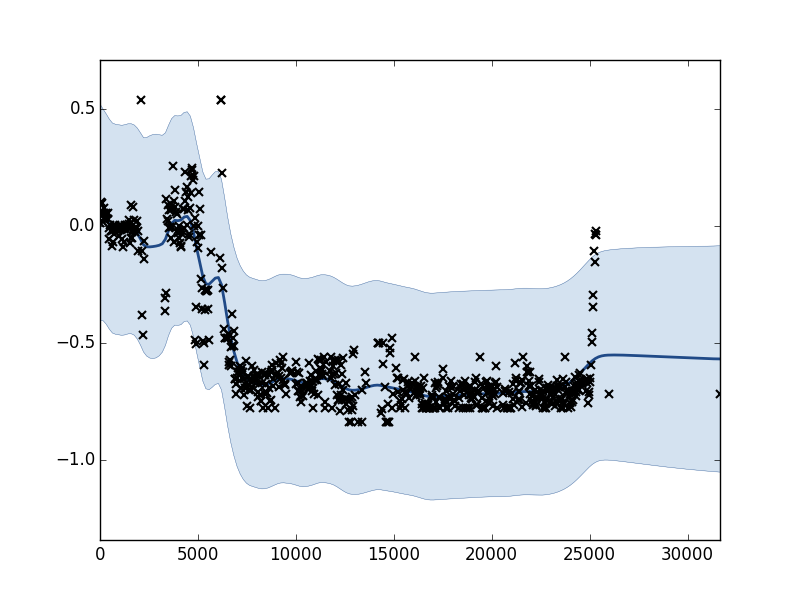
\includegraphics[width=230px,natwidth=665,natheight=361]{selected_GP/3056.csv_X.png}
  \caption{$x$-coordinate of Tag 3056 plotted against time. (with mean and variance derived from the Gaussian Process model)}
  \label{fig:GP1}
\end{figure}

\subsection{2.3  Important Requirements}

A requirement of our task is a Gaussian Process model with multiple outputs, namely the $x$, $y$ and $z$ coordinates of each person. Our experiment uses a simple multivariate model which applies a separate GP to each dimension, thus assuming statistical independence between the three dimensions. However, the actual coordinates are likely to have a significant correlation and structure. Thus, one possible improvement is to construct GP models with correlated output, by passing the independent GP priors through a function, such as multi-class classification, as described in a paper by {\it Antoni B.Chan} on the topic of Multivariate Generalized Gaussian Process Models. \\

As we use time-series data for the Gaussian Process, there are potentially a large amount of data points, especially for time periods that last multiple days. Thus the efficiency of the algorithm is important. As we construct separate Gaussian Distributions for each person, the computations can be distributed over multiple machines.

\subsection{2.4  Interpreting Outputs}

After modelling the trajectories of each person as a function of time, point of time $T$, for each person $i$, we can determine the mean vector $\boldsymbol{\mu}$ and covariance matrix $K$ of the person's $x,y,z$ coordinates. Let $U_i$ be a random variable denoting the position $(x,y,z)$ of person $i$. Each $U_i$ can then be expressed as a trivariate normal distribution $U_i \sim \mathcal{N}(\boldsymbol{\mu},K)$.\\

To compute the expected amount of people in a region $R$, we define the indicator variables for each $i \in \{1,2,\cdots,n\}$:
\begin{center}
$X_i =
\begin{cases}
    1 &\text{if user }i\text{ is in region R}\\
    0 &\text{otherwise}
\end{cases}$
\end{center}
The expected value of $X_i$, is equal to the probability of person $i$ being in region $R$, which is computed as $\int_R p_i(x,y,z)dV$, where $p_i(x,y,z)$ is the probability density function of $U_i$. Thus, the total number of people in region $R$ is $\sum_{i=1}^n X_i$, with an expected value:
\begin{center}
$\displaystyle E[\sum_{i=1}^n X_i] = \sum_{i=1}^n E[X_i] = \sum_{i=1}^n \int_V p_i(x,y,z)dV$.
\end{center}

We note that since only a fraction of the people in the crowd is used in the data, the final value needs to be scaled accordingly to represent the total number of people within the region.

Thus, using simple integrations over regions, we can compute the expected number of people in each region. The outputs of the GP model are useful in helping human users or experts to use a small sample of people in the data to predict the population density of a particular area at any point of time. The idea is that a small group of people can be tagged, and they will conduct their activities as per normal. By getting the data of their movements and passing it through the GP model, one can predict the expected population density of a particular area at any point of time.

\section{3.  Technical Approach}

In our experiment, we do a simplified version of our model, using independent GP models for each of the axes $x$, $y$ and $z$, thus assuming the covariances between any two variables to be $0$. \\

\subsection{3.1  Implementation Details}

In order to support the use of big data and the data of different demographics, we experimented with several families of kernel functions including the Radial Basis function (RBF), Exponential function, Matern52, Matern32 and Multilayer Perceptron (MLP). The experiments conducted involved varying their respective parameters such as noise values, relaxing or fixing constraints, changing initial values and inducing points and combining with various White and Bias kernels. Finally, the combination of kernel functions that yield consistent results as observed cross different samples from our dataset is selected to build our GP model for further application. In our case, we found out that MLP with a bias is the most effective way of representing the big data that we have.\\

We extract the X, Y and Z coordinates from the position data and perform the regression against the timestamps provided in the dataset. We also generate a common set of timestamps to predict the user movements against, in which we generate the mean and variance from the output of the GP we had earlier regressed. \\

The Sheffield GPy library was used for the GP modelling and regression. Python offers many useful libraries like Scipy, Numpy and Pandas, which provide useful data analysis tools for our dataset, as well numerical analysis tools like numerical integration.\\

The two methods we have chosen to regress our model are either the Stochastic Variational Inference method using the climin module or the AdaDelta rule and direct optimization using BFGS method. Through observing the results from several samples of our dataset, the latter is found to provide more desirable results and more suitable to be used in our propose application. Therefore, it is chosen for further experiments. Figure \ref{fig:GP1} and Figure \ref{fig:GP2} show the output of two such regressions for users 3056 and 3064.

\begin{figure}[h!]
  \centering
    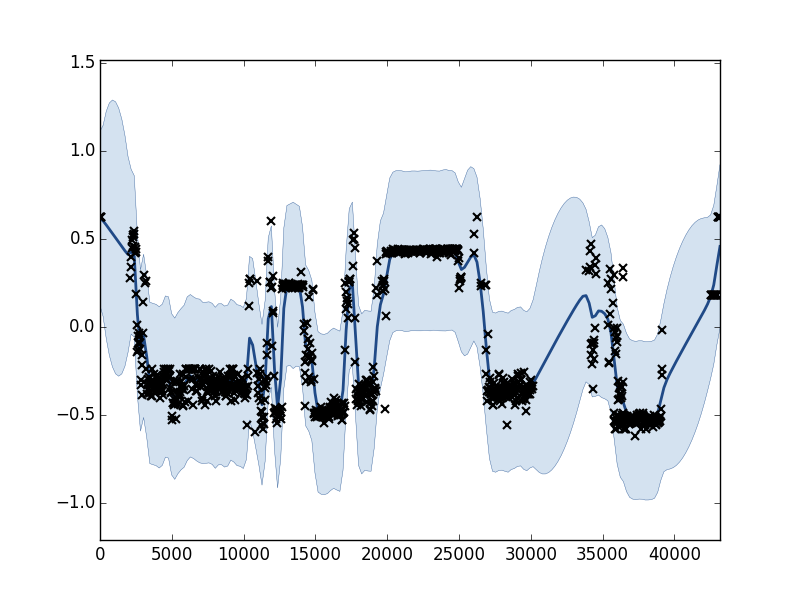
\includegraphics[width=230px,natwidth=665,natheight=361]{selected_GP/3064.csv_Y.png}
  \caption{$y$-coordinate of Tag 3064 plotted against time. (with mean and variance derived from the Gaussian Process model)}
  \label{fig:GP2}
\end{figure}

\subsection{3.2  Additional Insights}

We use a heteroscedastic model that works the same way as a GP model. However, this model allows the use of different variances for the noise terms of the observations, $\epsilon_i \sim N(0, \sigma_i^2)$, giving different weights to each observation. Therefore, it serves to fit observations with smaller noise and choose to ignore those with larger noise. \\

By experimenting with different kernel functions, we obtain the final GP model using a linear combination of a Multilayer Perceptron (MLP) and a constant Bias as kernel function as they consistently output acceptable results for regressions on our dataset. MLP, also known as arc sine kernel or neural network kernel, can be optimized to represent a complex non-linear function. \\

We also noticed that the number of dimensions the dataset have will affect the computational efficiency as GP is not computationally efficient in high dimensional spaces. Since our dataset only consists of a few dimensions, each GP model takes less than a minute to compute on average with the longest taking approximately 3 minutes.\\

Several types of GP models were experimented with, including Stochastic Variance Gaussian Processes and Sparse Gaussian Processes. We also performed experiments with all the different types of kernels provided by the GPy library, including linear kernel and white kernel. We also tweaked the input parameters, such as the variance of the kernels to experiment with the data. The GP model-variant that we proposed has the co-variance matrix and mean that fits the data the best. \\

Be default we regress the $(x,y,z)$ coordinates of each individual as it is convenient to use and easy to understand (and integrate over). However, an issue with cartesian coordinates is that they may not be a very good model of crowd densities, especially for less open spaces. In wide open spaces, this is not an issue as individuals with similar cartesian coordinates are likely to be close to each other as well. However, in buildings with narrower corridors and tighter spaces, individuals with similar cartesian coordinates may actually be very far apart from each other. Figures \ref{fig:opspace1} and Figure \ref{fig:opspace2} illustrate this idea.

\begin{figure}[h!]
  \centering
    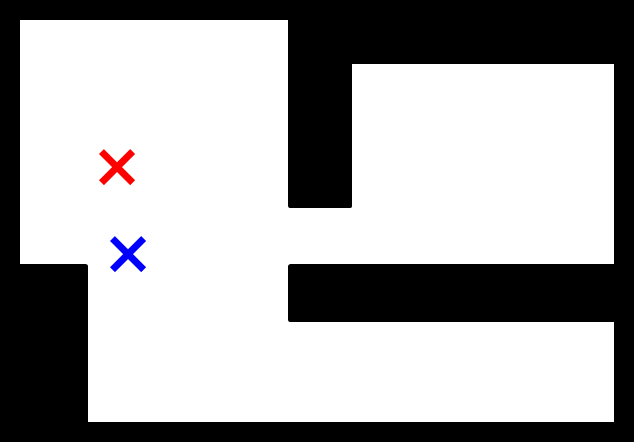
\includegraphics[width=150px,natwidth=634,natheight=442]{openspace1.png}
  \caption{Points with similar $x$ and $y$ coordinates in an open space}
  \label{fig:opspace1}
\end{figure}

\begin{figure}[h!]
  \centering
    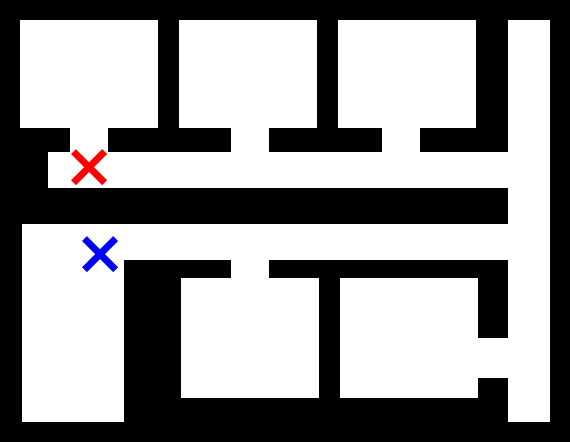
\includegraphics[width=150px,natwidth=570,natheight=402]{openspace2.png}
  \caption{Points with similar $x$ and $y$ coordinates in a less open space}
  \label{fig:opspace2}
\end{figure}

\subsection{3.3  Improvement}

To model less open spaces, we can use an alternative modelling, provided we know the layout of the area. Instead of using the cartesian coordinates of each user, we can use shortest path distances as the attributes instead. We first define a set of reference points at significant points $p_1,p_2,\cdots,p_k$ in the area. For each data point $d$, we compute the shortest paths $s_i$ from the data point to each of the reference points $p_i$. This is shown in Figure \ref{fig:spaths}. \\

We then use the same GP model as before using the values $s_i$ as the attributes. The advantage of using shortest paths as a metric is the geometry of the map has been abstracted out; two points with similar values of $s_i$ must be points that are close to each other. (given enough reference points)

\begin{figure}[h!]
  \centering
    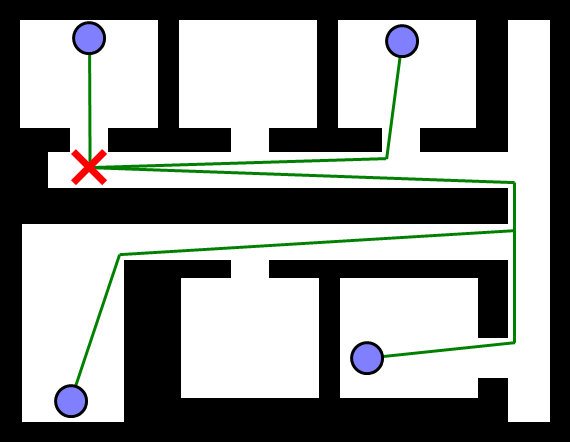
\includegraphics[width=150px,natwidth=570,natheight=442]{shortestpaths.png}
  \caption{The shortest paths from a data point to four reference points}
  \label{fig:spaths}
\end{figure}

We note that there are many available algorithms for quickly and accurately computing shortest paths within the area, if an accurate map (or floor plan) of the area is provided. However, it is important to note that with this formulation, the reference points must be carefully picked for a good prediction. (spread out, and preferably near the areas one is concerned about)\\

Integrations using the shortest path formulation will also be slightly more complex, as regions are now defined in terms of the path length to each of the reference points.

\section{4.  Experimental Evaluation}

\subsection{4.1  Real-World Dataset}

We test our approach using a Attendee Meta-Data (AMD) Hope RFID Dateset from which data is collected from 1224 hackers attending The Last HOPE Conference from 18-20 July 2008, located in Hotel Pennsylvania, New York City. The data set details the location of the people through the use of RFID badges that uniquely identify and track them across the conference space over the course of the conference. \\

This dataset was used as it has some convenient properties which allow us to construct an experiement to test our model. Firstly, the position data is usually taken at regular intervals of about $30$ seconds apart. Secondly, the data provided is exhaustive (as each attendee to the conference is tagged). This provides enough information to find the actual number of people in each region at any point of time, by simply counting the number of people within the region, within in a time window of $[t-15,t+15)$, where $t$ is the target point of time. 

\subsection{4.2  Experimental Setup}

In the experiment, the conference area is divided into $8\times 7 \times 2$ square regions (on the $x$,$y$ and $z$ axes respectively) that tile the conference area. $50$ time points are then picked randomly, while ensuring a minimum gap of $200$ seconds between any two time points, and that there are at least $300$ unique active tags near that time point. This is done to avoid testing on periods where no or few people are active, like during the night, as the event spans multiple days.\\

At each chosen time point $t$, the number of unique tags within each of the $112$ regions is counted. This is the actual data to be compared against. A small fraction (about $10\%$) of the people is then taken, the probability distributions of the people are generated using the GP model above, which is then used to estimate the number of people within each of the regions. \\

Figures \ref{fig:t1dist} to \ref{fig:t4dist} show the differences between the density plots between actual crowd densities and the predicted crowd densities from our experiment. One way of testing the quality of the fit is by observing how the distributions differ in the plotted charts below. A more empirical way of testing the quality of the fit is by taking the mean-squared error of the data between the actual and the predicted number of people. This can be compared across different models to test the accuracy of the prediction.

\begin{figure}[h!]
  \centering
    
\includegraphics[width=120px,natwidth=320,natheight=280]{selected_renders/0_1216437924.png}
  \caption{Actual density at $t=1216437924$, at floor $0$ of the event. ($z = 0$)}
  \label{fig:t1dist}
\end{figure}

\begin{figure}[h!]
  \centering
    
\includegraphics[width=120px,natwidth=320,natheight=280]{selected_renders/0_1216437924p.png}
  \caption{Predicted density at $t=1216437924$, at floor $0$ of the event. ($z = 0$)}
  \label{fig:t2dist}
\end{figure}

\begin{figure}[h!]
  \centering
    
\includegraphics[width=120px,natwidth=320,natheight=280]{selected_renders/1_1216440525.png}
  \caption{Actual density at $t=1216440525$, at floor $1$ of the event. ($z = 1.2$)}
  \label{fig:t3dist}
\end{figure}

\begin{figure}[h!]
  \centering
    
\includegraphics[width=120px,natwidth=320,natheight=280]{selected_renders/1_1216440525p.png}
  \caption{Predicted density at $t=1216440525$, at floor $1$ of the event. ($z = 1.2$)}
  \label{fig:t4dist}
\end{figure}

We note that using the simplified version of the Gaussian Model (statistically independent $x$, $y$ and $z$ coordinates), the probability distributions roughly approximate the crowd densities within each region in the event. Using this experiment setup, we can test the amount of improvement in the prediction when we apply modifications to the model, like using Multivariate Gaussian Processes to produce a full covariance matrix between $x$, $y$ and $z$, or using the shortest path formulation of the space.

\section{5.  Conclusion}

The goal of the current work is to present a representation that allows for modelling of crowds. We described a framework for modeling noisy, and unevenly sampled
data using the GP model and MLP with a bias constant, we demonstrated that our approach is able to represent the dataset we have as well as predict the population density at a given point of time.

\section{6. Main Roles of Each Member}
\begin{enumerate}
\item Wei Ling: Writing the report, research.
\item Nathan: Experimental setup and coding.
\item Lynnette / Thien: Setting up and experimenting with the Gaussian Process models
\item Shunhao: Problem formulation and modelling, mathematics, visualisations.
\end{enumerate}

\section{7.  References}

[1] Marco A. F. Pimentel, David A. Clifton, Lionel Tarassenko, `` Gaussian Process Clustering For The Functional Characterisation Of Vital-Sign Trajectories"
 in {\it 2013 IEEE International Workshop On Machine Learning For Signal Processing}, SEPT. 22–25, 2013, SOUTHAMPTON, UK. \\

[2] Antoni B. Chan, ``{ Multivariate Generalized Gaussian Process Models}" NOV. 03, 2013 \\

[3] M. Ebden, ``{ Gaussian Processes for Regression: A Quick Introduction}" AUG, 2008 \\


\end{document}
